\documentclass{article}

\usepackage{appendix}
\usepackage{mathtools}
\usepackage{graphicx}
\graphicspath{{./figures/}}
\usepackage{csvsimple}
\usepackage{longtable}
\usepackage{listings}

\author{Konstantinos Dadamis \\ 1002224}
\title{Artificial Intelligence 4 \\ Assessed Exercise Report}

\begin{document}

\maketitle

\section{Introduction}
\label{intro}

\subsection{Identification}
This document is the report for the assessed exercise of the Artificial Intelligence 4 (AI4) course. 

\subsection{Description of the Exercise}
\label{intro:descr}

For the purposes of this exercise, a system was developed for classifying audio signals into speech and silence. 
It included two parts: the Sensing and the Reasoning part. 
The Sensing part involved extracting features from audio signals and more specifically, the Energy, the Magnitude and Zero-Crossing Rate, while the Reasoning part involved using these features to classify the signals.
100 audio files, 300ms long, parts of telephone conversations, along with their samples were given to the students to test their system. 
Half of the audio files contained silence, while the other half contained speech.

\subsection{Description of the Document}

The document comprises~\ref{exp} sections and 2 appendices. 
A more detailed description of the problem in ``PEAS'' terms can be found in section~\ref{des}.
Section~\ref{the} contains the approaches adopted at the Sensing and Reasoning stages, while section~\ref{exp} consists of the experiments conducted.
Tables with extracted features from the files given can be found in appendix~\ref{prtab} and the code used for this exercise is located in appendix~\ref{code}.

\section{Design}
\label{des}

As mentioned in section~\ref{intro:descr}, for the purposes of this exercise, an agent was developed to classify audio signals into the Speech class and the Silence class.
When designing an agent, the task environment must be defined as clearly as possible.
The task environment can be defined with the ``PEAS'' description, i.e. the Performance measure, the Environment and the agent's Actuators and Sensors.

The performance measure defines the desirable behaviour of the agent.
This agent's desirable behaviour is mainly defined by its accuracy at detecting whether a particular audio samples file belongs to the Speech or the Silence class.
Lower accuracy means lower performance, but high accuracy means that the agent is of high quality.
Another performance measure is the speed at which it is able to classify the samples files.
%More?

One part of the agent's environment is the set of text files that it is interacting with. 
These files represent samples taken from audio files that need to be classified. 
They consist of integers separated by newline characters. 
Another part of the environment is the users who are using the classifier. 
The users are responsible for indicating the files which need to be classified as well as inputting some of the details of the files.

The actuator is the way the agent acts upon the environment.
Since the classifier does not have any other means to affect its environment, its only actuator is the output to the user's screen.
This output informs the user about how the classifier is trained and the outcome of the classification process. %delete is trained?

Finally, the sensor is the way the agent perceives the environment.
Since text files are input to the agent, two of the agent's sensors are the file reading and text decoding algorithms that are employed.
They are responsible for translating the text contained in the files into samples which are used by the agent.
In order to load files to the agent, certain methods need to be invoked. 
These methods have arguments which specify the names of the files, the duration of the actual audio file along with the time length of the window which should be used (explained in section~\ref{the}). 
As a result, the methods' arguments are also considered to be sensors.

\begin{table}[!h]

  \centering
  \begin{tabular}{ | p{.18\textwidth} || p{.16\textwidth} | p{.16\textwidth} | p{.16\textwidth} | p{.16\textwidth} | }
    \hline
    Agent Type & Performance Measure & Environment & Actuators & Sensors \\
    \hline
    Speech/Silence Classifier & 
    Accuracy, speed & 
    Set of audio samples files, users & 
    Display of results & 
    File input and text decoding algorithms, keyboard entry of filename, duration and window length \\
    \hline
  \end{tabular}
  \caption{``PEAS'' description of the task environment}
  \label{tab:peas}
\end{table}


\section{Theory}
\label{the}

The general approach adopted for building the classifier was to extract features from audio samples that we know the class they belong to and afterwards, use the features along with the known class to train a Naive Bayes Classifier.
After the classifier was built, the K-fold validation technique was used to validate the classifier.
The results of the experiments performed are located in section~\ref{exp}.

\subsection{Extracting features}

Audio signal short-term properties were used to train the classifier. 
In order to extract the properties from the audio samples, short-term analysis of the signals was used.
The outcomes of the analysis conducted were the Energy, the Magnitude and the Zero Crossing Rate (ZCR) of the signal.
A short-term property \(Q\) at the \(n\)th sample is defined by the following equation:

\[
  Q(n) = \sum_{k=-\infty}^{+\infty} F(s(k)) \times w(n-k) \quad (1)
\]

where \(s(k)\) is the sample of the audio file in position \(k\), \(F(s(k))\) is the function which is characteristic of the property and \(w(n-k)\) is the sliding window. 
Consequently, it is the convolution between \(F(s(k))\) and the window \(w(n-k)\).

The sliding window function is very useful for narrowing down the samples that are used for calculating the property at each position. 
Its main property is that it is zero-valued outside its length.
For the purposes of this exercise the rectangular window was used whose property is that it evaluates to 1 inside its length and zero otherwise.
Its equation is the following:

\[
  w(n) = \left\{ 
    \begin{array}{l l}
      0 & \quad n < 0 \\
      1 & \quad 0 \leq n \leq N-1 \\
      0 & \quad n \geq N
    \end{array} \right. \quad (2)
\]

where N is the length of the window.

By applying equation \((1)\) for the Energy (\(E(n)\)) with \(F(s(k)) = s^2(k)\) and the Magnitude (\(M(n)\)) with \(F(s(k)) = |s(k)|\):

\[
  E(n) = \sum_{k=-\infty}^{+\infty} s^2(k) \times w(n-k) \quad (3)
\]

\[
  M(n) = \sum_{k=-\infty}^{+\infty} |s(k)| \times w(n-k) \quad (4)
\]

In order to extract the ZCR, the \(sign(x)\) helper function is used to determine the sign of the signal and is defined as:

\[
  sign(x) = \left\{
    \begin{array}{l l}
      1 & \quad x \geq 0 \\
      0 & \quad x < 0
    \end{array} \right. \quad (5)
\]

Finally, the ZCR function (\(Z(n)\)) is derived by substituting \(F(s(k))\) with \(\frac{1}{2N}|sign(s(k)) - sign(s(k-1))|\):

\[
  Z(n) = \frac{1}{2N} \sum_{k=-\infty}^{+\infty} |sign(s(k)) - sign(s(k-1))| \times w(n-k) \quad (6)
\]

\subsection{Building the classifier}

As mentioned above, a Naive Bayes Classifier was built which classifies audio samples files into either Silence or Speech, i.e. defines whether they were taken from audio segments containing silence or speech.
In order to build the classifier, each audio file was represented by its Energy, Magnitude and ZCR properties.

A new audio file input to the classifier is of unknown class.
The class can be either Silence or Speech and there is no bias (like a coin toss).
As a result, the prior probability of its class being Silence is equal to the one being Speech, hence,

\[
  P(C=Sil) = P(C=Sp) = 0.5 \quad (7)
\]

The posterior is calculated by using Bayes theorem:

\[
  {\bf P}(C|E,M,Z) = \alpha{\bf P}(C)p(E,M,Z|C) \quad (8)
\]

In order to simplify the calculations, we assume that the Energy, the Magnitude and the ZCR are independent. Hence,

\[
  p(E,M,Z|C) = p(E|C)p(M|C)p(Z|C) \quad (9)
\]

\(p(E|C)\), \(p(M|C)\) and \(p(Z|C)\) are also assumed to be Gaussian which makes them easier to compute, since the probability for a Gaussian is:

\[
  p(x) = \frac{1}{\sqrt{2{\pi}\sigma^2}} e^{-\frac{(x-\mu)^2}{2\sigma^2}} \quad (10)
\]

where \(\mu\) and \(\sigma\) are the mean and the standard deviation of the Gaussian distribution.


The classification is done by comparing the probabilities \(P(C=Silence|E,M,Z)\) and \(P(C=Speech|E,M,Z)\). 
If \(P(C=Silence|E,M,Z) > P(C=Speech|E,M,Z)\), then the samples file is classified as Silence. 
Otherwise, it is classified as Speech. 
The comparison can be simplified by using equations (8), (7) and (9):

\begin{gather*}
  P(C=Sil|E,M,Z) > P(C=Sp|E,M,Z) \iff \\
  \iff \alpha{P}(C=Sil)p(E,M,Z|C=Sil) > \alpha{P}(C=Sp)p(E,M,Z|C=Sp) \iff \\
  \iff \alpha \times 0.5 \times p(E,M,Z|C=Sil) > \alpha \times 0.5 \times p(E,M,Z|C=Sp) \iff \\
  \iff p(E,M,Z|C=Sil) > p(E,M,Z|C=Sp) \iff \\
  \iff p(E|C=Sil)p(M|C=Sil)p(Z|C=Sil) > p(E|C=Sp)p(M|C=Sp)p(Z|C=Sp) \quad (11)
\end{gather*}

where the probabilities can be calculated as in equation (10).

\subsection{Validation}
\label{the_valid}

For the validation of the classifier, the K-fold validation technique was employed.
The set of files provided was split in K subsets and the validation was done in K iterations.
During each iteration one of the subsets was used for testing and the rest of the set was used for training the classifier. 
Afterwards, the trained classifier was used for predicting the class of each of the samples files in the test subset and the accuracy was calculated.
After K iterations, the overall accuracy of the classifier was measured.


\section{Experiments}
\label{exp}

\subsection{Extracting features} % sampling rate, how window was implemented, assumed sample=0 for k<0 and sign=0 for k<0

The set of audio samples files used were given by the instructors of the AI4 course.
It consists of 100 audio samples files, half of which are taken from silent audio segments, while the rest are taken from audio segments containing speech.
Each of the respective audio segments is 300ms long and since each data file contains 2400 samples, the sampling rate is 80kHz.
One of the assumptions that were made in the code was that the sample value at position \(k\) (\(s(k)\)) was considered to be equal to zero for \(k<0\). For the short-term analysis of the files, a window length of 30ms was used (Figure~\ref{fig:window}).

In addition, the Naive Bayes Classifier needed only one value to characterize each one of the properties of each file.
The average ZCR value of the file was chosen for the ZCR property.
As the Energy and Magnitude are figures of greater magnitude, the natural logarithm of the average value was chosen for these properties.
Tables~\ref{tab:sil} and~\ref{tab:sp} which contain the characteristic values extracted from the silence and speech files respectively are located in appendix~\ref{prtab}.

\begin{figure}[h!]
  \centering
  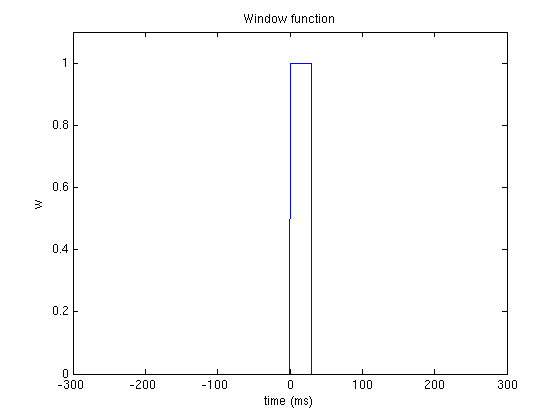
\includegraphics[width=0.9\textwidth]{window}
  \caption{Window function for window length of 30ms}
  \label{fig:window}
\end{figure}

\subsection{Building the classifier}

Before building the classifier, some diagrams were drawn to assure that the assumptions that were made in the theoretical part were true. 
Firstly, the Energy-Magnitude, Magnitude-ZCR and Energy-ZCR diagrams were drawn for all the files given (Figures~\ref{fig:e-m},~\ref{fig:m-z} and~\ref{fig:e-z} respectively). 
Figure~\ref{fig:e-m} shows that there is high correlation between Energy and Magnitude, but the other two diagrams indicate that the independence assumption we made was correct.

\begin{figure}[h!]
  \centering
  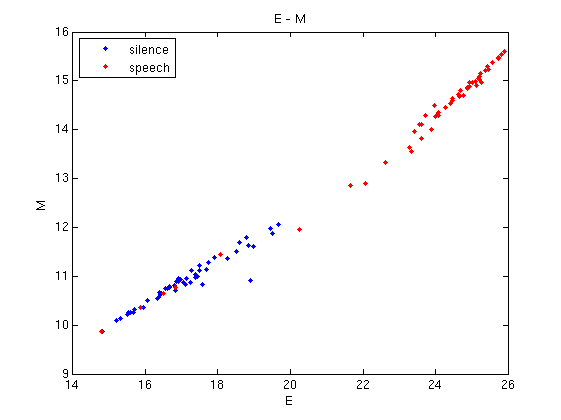
\includegraphics[width=0.9\textwidth]{e-m}
  \caption{Energy-Magnitude scatter plot}
  \label{fig:e-m}
\end{figure}
\begin{figure}[h!]
  \centering
  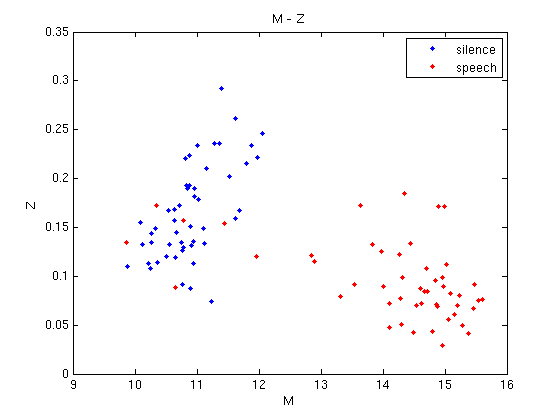
\includegraphics[width=0.9\textwidth]{m-z}
  \caption{Magnitude-ZCR scatter plot}
  \label{fig:m-z}
\end{figure}
\begin{figure}[h!]
  \centering
  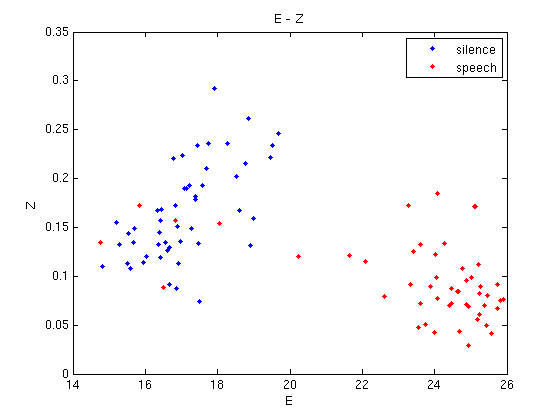
\includegraphics[width=0.9\textwidth]{e-z}
  \caption{Energy-ZCR scatter plot}
  \label{fig:e-z}
\end{figure} 

Secondly, the histograms for the Energy, Magnitude and ZCR values---separately for silence and speech---were also drawn to check whether their distribution is Gaussian or not (Figures~\ref{fig:histo_sil_e}, \ref{fig:histo_sil_m}, \ref{fig:histo_sil_z}, \ref{fig:histo_sp_e}, \ref{fig:histo_sp_m} and~\ref{fig:histo_sp_z}). At the Energy and Magnitude histograms of the speech class (Figures~\ref{fig:histo_sp_e} and~\ref{fig:histo_sp_m}), the distribution does not resemble a Gaussian one, but since the rest of the histograms appear to be Gaussian, we consider the assumption that they are all Gaussian distributions true.

\begin{figure}[h!]
  \centering
  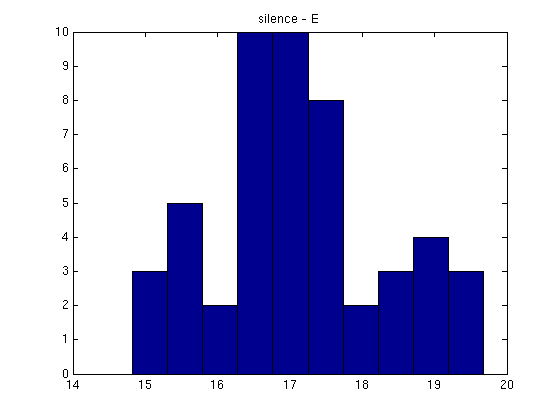
\includegraphics[width=0.9\textwidth]{histo_sil_e}
  \caption{Energy histogram for silence}
  \label{fig:histo_sil_e}
\end{figure} 
\begin{figure}[h!]
  \centering
  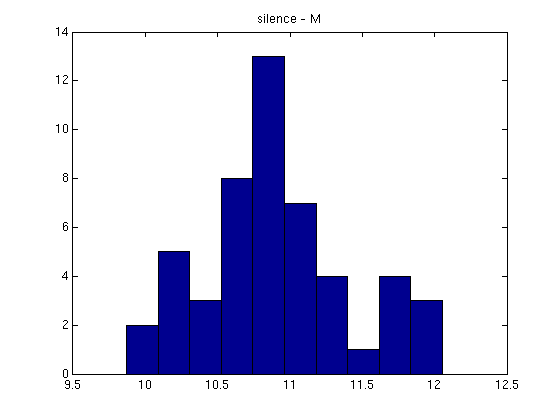
\includegraphics[width=0.9\textwidth]{histo_sil_m}
  \caption{Magnitude histogram for silence}
  \label{fig:histo_sil_m}
\end{figure} 
\begin{figure}[h!]
  \centering
  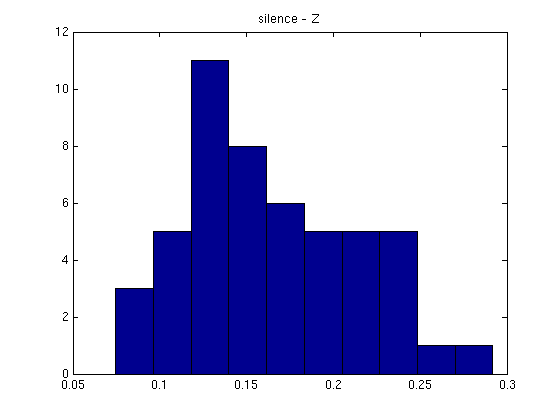
\includegraphics[width=0.9\textwidth]{histo_sil_z}
  \caption{ZCR histogram for silence}
  \label{fig:histo_sil_z}
\end{figure} 
\begin{figure}[h!]
  \centering
  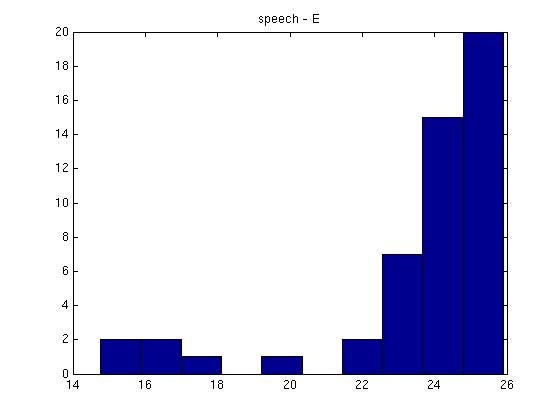
\includegraphics[width=0.9\textwidth]{histo_sp_e}
  \caption{Energy histogram for speech}
  \label{fig:histo_sp_e}
\end{figure} 
\begin{figure}[h!]
  \centering
  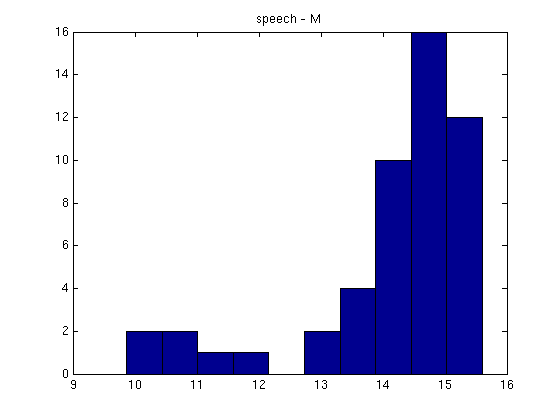
\includegraphics[width=0.9\textwidth]{histo_sp_m}
  \caption{Magnitude histogram for speech}
  \label{fig:histo_sp_m}
\end{figure} 
\begin{figure}[h!]
  \centering
  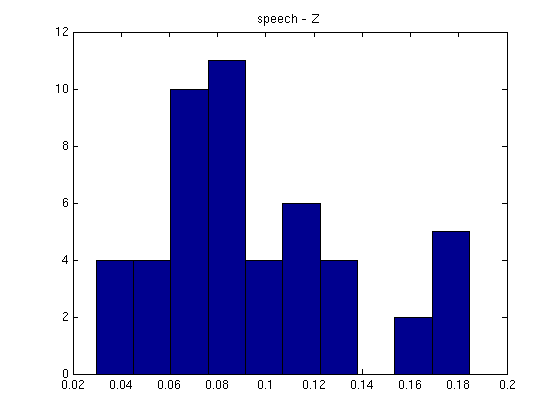
\includegraphics[width=0.9\textwidth]{histo_sp_z}
  \caption{ZCR histogram for speech}
  \label{fig:histo_sp_z}
\end{figure} 

\subsection{Validation}

As mentioned in subsection~\ref{the_valid}, the K-fold validation technique was employed.
For this exercise, K was considered to be equal to 10, so the set of files was split into 10 subsets, with each one containing 5 silence and 5 speech samples files.
The accuracy of the classifier during the 10 iterations fluctuated between 80\% and 100\%.
The agent performed 95 correct classifications and 5 misclassifications, so its overall accuracy is 95\%. 

The 5 samples files which were misclassified were 5 speech samples files: ``speech\_13.dat'', ``speech\_16.dat'', ``speech\_23.dat'', ``speech\_39.dat'' and ``speech \_40.dat''. % space?
By looking at the scatter plot diagrams in Figures~\ref{fig:e-m}, \ref{fig:m-z} and~\ref{fig:e-z}, we can realise why these misclassifications happened. 
There are 5 speech files which are consistently located in the areas where the silence files are gathered and these are the files which are causing the misclassifications.

\newpage

\appendix
\appendixpage

\section{Properties Tables}
\label{prtab}

\begin{longtable}{|c|c|c|c|} \hline
  File no. & Energy & Magnitude & ZCR \\\hline
  \csvreader[late after line=\\\hline]
            {silence_features.csv}{}
            {\thecsvrow & \csvcoli & \csvcolii & \csvcoliii}

            \caption{The silence files' properties}
            \label{tab:sil}
\end{longtable}

\newpage

\begin{longtable}{|c|c|c|c|} \hline
  File no. & Energy & Magnitude & ZCR \\\hline
  \csvreader[late after line=\\\hline]
            {speech_features.csv}{}
            {\thecsvrow & \csvcoli & \csvcolii & \csvcoliii}

            \caption{The speech files' properties}
            \label{tab:sp}
\end{longtable}

\section{Code Listings}
\label{code}

The code provided could be implemented in a more efficient way, but clarity of code was preferred over efficiency.

\subsection{calc\_features.m}
\lstinputlisting[language=Matlab]{calc_features.m}

\subsection{store\_features\_all.m}
\lstinputlisting[language=Matlab]{store_features_all.m}

\subsection{scatter\_plot\_features.m}
\lstinputlisting[language=Matlab]{scatter_plot_features.m}

\subsection{histo.m}
\lstinputlisting[language=Matlab]{histo.m}

\subsection{gaussian\_pdf.m}
\lstinputlisting[language=Matlab]{gaussian_pdf.m}

\subsection{get\_mean\_variance.m}
\lstinputlisting[language=Matlab]{get_mean_variance.m}

\subsection{k\_fold.m}
\lstinputlisting[language=Matlab]{k_fold.m}




\end{document}
